%
% This is an example file and is hereby explicitly put in the
% public domain.
%
\documentclass[ppgc,diss,english]{iiufrgs}
% Para usar o modelo, deve-se informar o programa e o tipo de documento.
% Programas :
%   * cic       -- Graduação em Ciência da Computação
%   * ecp       -- Graduação em Ciência da Computação
%   * ppgc      -- Programa de Pós Graduação em Computação
%   * pgmigro   -- Programa de Pós Graduação em Microeletrônica
%
% Tipos de Documento:
%   * tc                -- Trabalhos de Conclusão (apenas cic e ecp)
%   * diss ou mestrado  -- Dissertações de Mestrado (ppgc e pgmicro)
%   * tese ou doutorado -- Teses de Doutorado (ppgc e pgmicro)
%   * ti                -- Trabalho Individual (ppgc e pgmicro)
%
% Outras Opções:
%   * english    -- para textos em inglês
%   * openright  -- Força início de capítulos em páginas ímpares (padrão da
%                   biblioteca)
%   * oneside    -- Desliga frente-e-verso
%   * nominatalocal -- Lê os dados da nominata do arquivo nominatalocal.def


% Use unicode
\usepackage[utf8]{inputenc}   % pacote para acentuação

% Necessário para incluir figuras
\usepackage{graphicx}           % pacote para importar figuras
\usepackage{tikz}

\usepackage{nicefrac}       % compact symbols for 1/2, etc.
\usepackage{amsfonts}       % blackboard math symbols
\usepackage{xspace}
\usepackage{amsmath}
\usepackage{amsthm}
\usepackage{amssymb}
\usepackage{algorithm}
\usepackage{algpseudocode}

% \usepackage{times}              % pacote para usar fonte Adobe Times
 \usepackage{palatino}
% \usepackage{mathptmx}          % p/ usar fonte Adobe Times nas fórmulas

\usepackage[alf,abnt-emphasize=bf]{abntex2cite}	% pacote para usar citações abnt


\providecommand{\multiset}[1]{\ensuremath{\{\!\!\{#1\}\!\!\}}}
\providecommand{\sas}{\ensuremath{\text{SAS}^{+}}\xspace}
\providecommand{\strips}{STRIPS\xspace}
\providecommand{\astar}{\ensuremath{\text{A}^{*}}\xspace}
\providecommand{\gbfs}{\ensuremath{\text{GBFS}}\xspace}
\providecommand{\wida}{\ensuremath{\text{W-IDA}^{*}}\xspace}
\providecommand{\ida}{\ensuremath{\text{IDA}^{*}}\xspace}
\providecommand{\hvalue}[1]{\ensuremath{h^{#1}}\xspace}
\providecommand{\hstarp}[1]{\ensuremath{h^*({#1})}\xspace}
\providecommand{\hff}{\hvalue{\text{FF}}}
\providecommand{\hgc}{\hvalue{\text{GC}}}
\providecommand{\hstar}{\hvalue{*}}
\providecommand{\hlmc}{\hvalue{\text{lm-c}}}
\providecommand{\hmax}{\hvalue{\text{max}}}
\providecommand{\hadd}{\hvalue{\text{add}}}
\providecommand{\h}{$h$\xspace}
\providecommand{\hnn}{$\hat h$\xspace}
\providecommand{\hnrsl}{$\hat h^{\text{N-RSL}}$\xspace}
\providecommand{\hboot}{$\hat h^{\text{Boot}}$\xspace}
\providecommand{\hgc}{\hvalue{\text{gc}}}
\providecommand{\hhgn}{\hvalue{\text{HGN}}}
\providecommand{\unit}{/1\xspace}
\providecommand{\sui}{\text{SUI}\xspace}
\providecommand{\sai}{\text{SAI}\xspace}
\providecommand{\rw}{{RW}\xspace}
\providecommand{\bfs}{{BFS}\xspace}
\providecommand{\dfs}{{DFS}\xspace}
\providecommand{\bfsrw}{\text{FSM}\xspace}
\providecommand{\nn}{{NN}\xspace}
\providecommand{\fssp}{{FS}\xspace}
\providecommand{\bssp}{{BS}\xspace}
\providecommand{\hnnrs}{$\hat h{^{20\%}_\text{\meanfx}}$\xspace}
\providecommand{\hnnrsfifty}{$\hat h{^{50\%}_\text{\meanfx}}$\xspace}
\providecommand{\hffexp}{$h^{FF}_{exp}$}
\providecommand{\hgcexp}{$h^{GC}_{exp}$}
\providecommand{\hnnbase}{$\hat h_{0}$\xspace}
\providecommand{\hnnbfs}{$\hat h_{\text{bfs}}$\xspace}
\providecommand{\hnndfs}{$\hat h_{\text{dfs}}$\xspace}
\providecommand{\hnnrw}{$\hat h_{\text{rw}}$\xspace}
\providecommand{\hnnbfsrw}{$\hat h_\text{fsm}$\xspace}
\providecommand{\hnnbfsrwl}[1]{\ensuremath{\hat h_{#1}}\xspace}
\providecommand{\hnnnomutex}{\ensuremath{\hat h^{'}}\xspace}
\providecommand{\hnnnomutexl}[1]{\ensuremath{\hat h^{'}_{#1}}\xspace}
\providecommand{\hnnrsp}[1]{\ensuremath{\hat h_\text{fsm}/^{#1\%}_{\text{RS}}}\xspace}
\providecommand{\hnnrslp}[2]{\ensuremath{\hat h_\text{fsm}^{#1}/^{#2\%}_{\text{RS}}}\xspace}
\providecommand{\define}[1]{#1}
\providecommand{\facts}{\ensuremath{L_F}\xspace}
\providecommand{\meanfx}{\ensuremath{L_{\overline{F}}}\xspace}
\providecommand{\default}{\ensuremath{L_{200}}\xspace}
\providecommand{\distfarthest}{\ensuremath{d^*}\xspace}
\providecommand{\po}[1]{\ensuremath{\hat po^{#1}}\xspace}
\providecommand{\pot}[1]{\ensuremath{po^{#1}}\xspace}
\providecommand{\pog}{\po{\text{G}}}
\providecommand{\pofsm}{\po{\text{B}}}
\providecommand{\pogthresh}{\po{\text{G-thresh}}}
\providecommand{\pogmax}{\po{\text{G-max}}}
\providecommand{\popfa}{\po{\text{PFA}}}
\providecommand{\popfo}{\po{\text{PFO}}}
\providecommand{\postar}{\po{*}}
\providecommand{\postartable}{\pot{*}}
\providecommand{\pogstar}{\po{\text{G}^*}}
\providecommand{\pogstarthresh}{\po{\text{OPT-thresh}}}
\providecommand{\pogstarmax}{\po{\text{OPT-max}}}
\providecommand{\popf}{\po{\text{PF}}}
\providecommand{\poff}{\pot{\text{FF}}}
\providecommand{\pogc}{\po{\text{GC}}}

%% mathematical definitions
\ifcsname dom\endcsname\else\DeclareMathOperator{\dom}{Dom}\fi
\DeclareMathOperator{\pre}{pre}
\DeclareMathOperator{\eff}{eff}
\DeclareMathOperator{\sucs}{succ}
\DeclareMathOperator{\pred}{pred}
\DeclareMathOperator{\functioninitial}{initial\_state}
\DeclareMathOperator{\functiongoal}{goal\_condition}
\DeclareMathOperator{\mutex}{mutex}
\DeclareMathOperator{\del}{del}
\DeclareMathOperator{\add}{add}
\ifcsname R\endcsname\else\newcommand{\R}{\ensuremath{\mathbb{R}}}\fi


\usepackage[textsize=tiny,colorinlistoftodos,prependcaption]{todonotes}

\newcommand{\mr}[2][noinline]{\todo[#1,fancyline,color=blue!20]{#2}}
\newcommand{\mri}[2][inline]{\todo[#1,fancyline,color=blue!20]{#2}}

\newcommand{\agp}[2][noinline]{\todo[color=orange!60,linecolor={orange!100},#1,fancyline,author=André]{#2}}
\newcommand{\agpi}[2][inline]{\todo[color=orange!60,linecolor={orange!100},#1,fancyline,author=André]{#2}}

\newcommand{\pp}[2][noinline]{\todo[color=purple!50,linecolor={purple!100},#1,fancyline,author=Pedro]{#2}}
\newcommand{\ppi}[2][inline]{\todo[color=purple!50,linecolor={purple!100},#1,fancyline,author=Pedro]{#2}}


%
% Informações gerais
%
\title{Discovering and Learning Preferred Operators for Classical Planning with Neural Networks}
\translatedtitle{Aprendizado de Operadores Preferidos em Planejamento Clássico}

\author{Minini}{Pedro Probst}
% alguns documentos podem ter varios autores:
%\author{Flaumann}{Frida Gutenberg}
%\author{Flaumann}{Klaus Gutenberg}

% orientador e co-orientador são opcionais (não diga isso pra eles :))
\advisor[Prof.~Dr.]{Ritt}{Marcus}
\coadvisor[Prof.~Dr.]{Pereira}{André Grahl}

% a data deve ser a da defesa; se nao especificada, são gerados
% mes e ano correntes
%\date{maio}{2001}

% o local de realização do trabalho pode ser especificado (ex. para TCs)
% com o comando \location:
%\location{Itaquaquecetuba}{SP}

% itens individuais da nominata podem ser redefinidos com os comandos
% abaixo:
% \renewcommand{\nominataReit}{Prof\textsuperscript{a}.~Wrana Maria Panizzi}
% \renewcommand{\nominataReitname}{Reitora}
% \renewcommand{\nominataPRE}{Prof.~Jos{\'e} Carlos Ferraz Hennemann}
% \renewcommand{\nominataPREname}{Pr{\'o}-Reitor de Ensino}
% \renewcommand{\nominataPRAPG}{Prof\textsuperscript{a}.~Joc{\'e}lia Grazia}
% \renewcommand{\nominataPRAPGname}{Pr{\'o}-Reitora Adjunta de P{\'o}s-Gradua{\c{c}}{\~a}o}
% \renewcommand{\nominataDir}{Prof.~Philippe Olivier Alexandre Navaux}
% \renewcommand{\nominataDirname}{Diretor do Instituto de Inform{\'a}tica}
% \renewcommand{\nominataCoord}{Prof.~Carlos Alberto Heuser}
% \renewcommand{\nominataCoordname}{Coordenador do PPGC}
% \renewcommand{\nominataBibchefe}{Beatriz Regina Bastos Haro}
% \renewcommand{\nominataBibchefename}{Bibliotec{\'a}ria-chefe do Instituto de Inform{\'a}tica}
% \renewcommand{\nominataChefeINA}{Prof.~Jos{\'e} Valdeni de Lima}
% \renewcommand{\nominataChefeINAname}{Chefe do \deptINA}
% \renewcommand{\nominataChefeINT}{Prof.~Leila Ribeiro}
% \renewcommand{\nominataChefeINTname}{Chefe do \deptINT}

\renewcommand{\nominataReit}{Prof.~Carlos Andr{\'e} Bulh{\~o}es}
%\renewcommand{\nominataReitname}{Rector}
\renewcommand{\nominataPRCA}{Prof.~Patricia Pranke}
%\renewcommand{\nominataPRCAname}{Vice-Rector}
\renewcommand{\nominataPRAPG}{Prof.~J{\'u}lio Ot{\'a}vio Jardim Barcellos}
%\renewcommand{\nominataPRAPGname}{Dean of Graduate Studies}
\renewcommand{\nominataDir}{Prof.~Carla Maria Dal Sasso Freitas}
%\renewcommand{\nominataDirname}{Director of the Institute of Informatics}
\providecommand{\nominataCoord}{Prof.~Alberto Egon Schaeffer Filho}
%\providecommand{\nominataCoordname}{Coordinator of the PPGC}
\renewcommand{\nominataBibchefe}{Alexsander Borges Ribeiro}
%\renewcommand{\nominataBibchefename}{Chief Librarian of the Institute of Informatics}

% A seguir são apresentados comandos específicos para alguns
% tipos de documentos.

% Relatório de Pesquisa [rp]:
% \rp{123}             % numero do rp
% \financ{CNPq, CAPES} % orgaos financiadores

% Trabalho Individual [ti]:
% \ti{123}     % numero do TI
% \ti[II]{456} % no caso de ser o segundo TI

% Monografias de Especialização [espec]:
% \espec{Redes e Sistemas Distribuídos}      % nome do curso
% \coord[Profa.~Dra.]{Weber}{Taisy da Silva} % coordenador do curso
% \dept{INA}                                 % departamento relacionado

%
% palavras-chave
% iniciar todas com letras maiúsculas
%
\keyword{Classical planning}
\keyword{Heuristic search}
\keyword{Preferred operators}
\keyword{Machine learning}

%
% palavras-chave na lingua estrangeira
% iniciar todas com letras maiúsculas
%
\translatedkeyword{Planejamento clássico}
\translatedkeyword{Busca heurística}
\translatedkeyword{Operadores preferidos}
\translatedkeyword{Aprendizado de máquina}


%
% inicio do documento
%
\begin{document}

% folha de rosto
% às vezes é necessário redefinir algum comando logo antes de produzir
% a folha de rosto:
% \renewcommand{\coordname}{Coordenadora do Curso}
\maketitle

% dedicatoria
\clearpage
\begin{flushright}
\mbox{}\vfill
{\sffamily\itshape
    ``All this from a slice of gabagool?''\\}
--- \textsc{Tony Soprano}
\end{flushright}

% agradecimentos
\chapter*{Acknowledgements}
TODO.

% abstract in english
\begin{abstract}
In a planning task, an agent must choose the most appropriate action from a potentially large set of actions at each step. Symbolic-based planners employ preferred operators to reduce the number of actions significantly. This work presents a method for sampling and learning preferred operators, ensuring their applicability across the entire state space of a planning task. We demonstrate that these learned preferred operators outperform the current best symbolic-based approach.
We aim to identify ideal preferred operators, which are situated along the shortest paths leading to some goal. However, due to the huge size of search state spaces, we introduce a novel sampling strategy tailored for extracting preferred operators. Our research shows that high-quality preferred operators can be obtained from a sample set covering only a fraction of the state space. Furthermore, a small neural network trained on these samples can effectively approximate ideal preferred operators for tasks involving numerous states.
To gain insights into this new category of preferred operators, we conduct controlled experiments: we systematically compare them to baselines, evaluate the effectiveness of preferred operators learned from various sample sizes, and assess their performance when combined with different heuristic functions.
\end{abstract}

% abstract in portuguese
\begin{translatedabstract}
Em uma tarefa de planejamento, um agente deve escolher a ação mais adequada de um conjunto potencialmente grande de ações em cada passo. Planejadores simbólicos empregam operadores preferidos para reduzir significativamente o número de ações. Este trabalho apresenta um método para amostragem e aprendizagem de operadores preferidos, garantindo sua aplicabilidade em todo o espaço de estados de uma tarefa de planejamento. Demonstramos que esses operadores preferidos aprendidos superam a melhor abordagem simbólica atual.
Nosso objetivo é identificar os operadores preferidos ideais, que estão situados ao longo dos caminhos mais curtos que levam a algum objetivo. No entanto, devido ao enorme tamanho dos espaços de estado, apresentamos uma nova estratégia de amostragem adaptada para extrair operadores preferidos. Nossa pesquisa mostra que operadores preferidos de alta qualidade podem ser obtidos de um conjunto de amostras que abrange apenas uma fração do espaço de estados. Além disso, uma pequena rede neural treinada nessas amostras pode aproximar com eficácia os operadores preferidos ideais para tarefas que envolvem vários estados.
Para obter uma compreensão mais aprofundada sobre essa nova categoria de operadores preferidos, realizamos experimentos controlados: nós os comparamos sistematicamente com \textit{baselines}, avaliamos a eficácia dos operadores preferidos aprendidos com vários tamanhos de amostra e avaliamos seu desempenho quando combinados com diferentes funções heurísticas.
\end{translatedabstract}

% lista de abreviaturas e siglas
% o parametro deve ser a abreviatura mais longa
% A NBR 14724:2011 estipula que a ordem das abreviações
% na lista deve ser alfabética (como no exemplo abaixo).
\begin{listofabbrv}{SPMD}
        \item[BSS] Backward State Space
        \item[DTG] Domain Transition Graph
        \item[FSS] Forward State Space
        \item[FF] Fast-Forward
        \item[GBFS] Greedy Best-First Search
        \item[IPC] International Planning Competition
        \item[NN]  Neural Network
        \item[PDDL] Planning Domain Definition Language
        \item[\sas] Simplified Action Structures Plus
        \item[SD] Standard Deviation
        \item[STRIPS] Stanford Research Institute Problem Solver
\end{listofabbrv}

\begin{listofsymbols}{$\alpha\beta\pi\omega$}
       \item[\h] Heuristic
       \item[\hstar] Optimal heuristic
       \item[\hnn] Learned heuristic
       \item[\hadd] Add heuristic
       \item[\hff] FF heuristic
       \item[\hgc] Goal-count heuristic
       \item[\poff] FF preferred operator
       \item[\pog] Learned preferred operator
\end{listofsymbols}

\listoffigures

\listoftables

\listofalgorithms

\tableofcontents

%
% - - - - - - - - - - - - - - - -- - - - - -
% intro
% - - - - - - - - - - - - - - - -- - - - - -
% introduce the problem,
% show why the problem is interesting,
% and how we attack it
%
\chapter{Introduction}

This work represents the first step on learning preferred operators with neural networks. Preferred operators are used in conjunction with heuristic functions and assist the search by reducing the number of expanded states when solving a planning task.

\section{Planning}
Planning involves determining a series of operators (or actions) that transitions a given initial state to a desired goal state~\cite{Lipovetsky/2014}.
In a classical planning task, the initial state serves as the starting point for an agent. The agent acts in a fully-observable environment, i.e., with access to all relevant information of the current state of the world, such as the positions of objects and the values of variables. The objective of the agent is to fulfill a specific goal condition. This is achieved by using deterministic operators to modify the current state of the world. A solution plan for the planning task can be defined as a sequence of operators that, when applied to the initial state, successfully satisfy the goal condition. The process of state expansion involves the application of all relevant operators to a given state, thereby generating its successor states.

For example, in a Blocks World task, consider the initial state (left) and the goal state (right) shown in Figure \ref{fig:intro-blocks}. The agent needs to apply a sequence of operators to reach the goal state from the initial state. We can define operators such as ``pick up block X'', ``put block X on block Y'', and ``put block X on the table.'' In this example, the agent can find one of the possible plans by applying the following operators: pick up block C, put block C on the table, pick up block B, put block B on block C, and put block A on block B.

\begin{figure}[ht]
\captionsetup{skip=5pt} % the original spacing looks ugly as f* so I adjusted it a little bit
\caption{Initial state (left) and goal state (right) of a Blocks World task.}
\centering
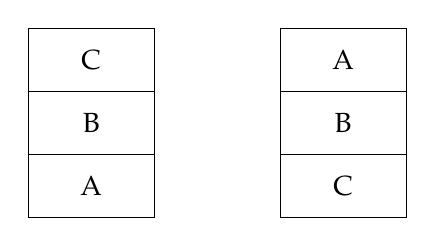
\begin{tikzpicture}[scale=0.8]
  % Initial configuration
  \draw (0,0) rectangle (2,1) node[midway] {A};
  \draw (0,1) rectangle (2,2) node[midway] {B};
  \draw (0,2) rectangle (2,3) node[midway] {C};

  % Goal configuration
  \draw (4,0) rectangle (6,1) node[midway] {C};
  \draw (4,1) rectangle (6,2) node[midway] {B};
  \draw (4,2) rectangle (6,3) node[midway] {A};
\end{tikzpicture}
\label{fig:intro-blocks}
\end{figure}

Planning tasks are solved by planners, which are software systems designed to find plans for given planning problems. Planners employ various algorithms and techniques to explore the search space of possible operators and states in order to find an optimal or satisfactory plan. Planners typically take as input a formal representation of the planning problem, including the initial state, goal condition, and a set of available operators. The formal representation of a planning task can be specified using various notations.

\section{Heuristic Search}
To solve planning tasks, planners commonly use a best-first search algorithm, which uses a function~$f$ to guide the search. The function $f$ combines the current cost $g(s)$ of a partial sequence of operations initiated from the initial state and reaching state $s$, along with a heuristic function $h(s)$ that provides an estimate of the cost-to-goal (also known as heuristic value or $h$-value) from state $s$. For example, \astar search is guided by $f(s)=g(s)+h(s)$~\cite{hart-et-al-ieeessc1968}, and greedy best-first search (\gbfs) is guided only by $f(s)=h(s)$~\cite{doran-michie-rsl1966}. In general, best-first search algorithms prove more effective when the heuristic function~$h$ better approximates the optimal heuristic function~\hstar.

%In particular, GBFS organizes states in a priority queue ordered by their cost-to-goal estimate, which is provided by the heuristic function. By expanding states with the lowest cost-to-goal estimate, GBFS finds a solution.
Various domain-independent heuristics efficiently calculate the cost-to-goal estimate of a state using domain logic, which includes specific information that aids in reasoning about operators and rules, such as mutexes indicating impossible states. Examples include delete relaxation~\cite{Hoffmann.Nebel/2001}, landmarks~\cite{hoffmann-et-al-jair2004,Karpas.Domshlak/2009}, critical paths~\cite{haslum-geffner-aips2000}, and state equation~\cite{bonet-ijcai2013}.

\section{Preferred Operators}
Preferred operators are used in conjunction with heuristic functions and can aid planners in reducing the number of expanded states during a search process~\cite{Helmert/2006,Richter.Helmert/2009}. Intuitively, preferred operators generate successor states that are closer to the goal. By prioritizing the expansion of states generated by preferred operators, planners benefit from additional guidance, often resulting in a higher success rate for solving tasks compared to only relying on the heuristic function. Learning preferred operators shares similarities with learning policies, as both involve the selection of actions that are more likely to result in desirable outcomes. The existing methods for identifying preferred operators are currently limited to symbolic-based (also called as logic-based) approaches. The most effective approach used at present involves using the preferred operators calculated alongside the Fast-Forward (FF) heuristic~\cite{Hoffmann.Nebel/2001}, as implemented in the Fast Downward planning system~\cite{Helmert/2006}. Preferred operators are particularly beneficial in competitive scenarios, as they maximize the number of solved tasks (coverage). Planners incorporating preferred operators emerged as winners in the satisficing track of the International Planning Competition (IPC) in 2004, 2008, 2011, and 2018~\cite{Helmert/2006,Richter.lama.etal/2011,Richter.lama.etal/2011,Seipp-fast.etal/2018}.

\section{Deep Learning}
Deep learning, as described by~\citet{Goodfellow.etal/2016}, is a subfield of machine learning that focuses on the design and training of neural networks (NNs) with multiple layers. It revolves around the concept of learning hierarchical representations of data, where each layer in the network progressively extracts more complex and abstract features. Through the use of deep neural networks, deep learning algorithms can automatically discover and capture intricate patterns from large-scale datasets in a varity of tasks, including image classification, speech recognition, natural language processing, and more.

Deep learning models can learn in different ways. This study focuses on supervised learning, which involves using labeled datasets to classify or make predictions. In this case, a dataset used to train an NN can be represented as multiple pairs in the format $(y, x)$. Here, the target $y$ refers to the desired output or label associated with a specific input instance $x$. Deep learning models can effectively learn and generalize from the provided labeled data to make accurate predictions or classify new, unseen inputs.

\section{Learning in Planning}
In recent years, interest in using NNs to learn heuristic functions~\cite{Ferber.etal/2020a,Yu.etal/2020,Shen.etal/2020,Ferber.etal/2022,OToole/2022} or policies~\cite{Toyer.etal/2018,Toyer.etal/2020,Stahlberg.etal/2022} to solve planning tasks has increased. For supervised methods, the general approach is to generate a set of samples as pairs of states and cost-to-goal values and use them to train a neural network. However, it is challenging to learn effective heuristic functions, since (a) state spaces tend to grow exponentially in size as the amount of information needed to describe them increases, but the portion of the state space that we can actually sample is relatively small, (b) symbolic-based heuristics can be applied to any domain, while learned heuristics are hard to transfer, and (c) learned heuristics are generally slow to compute, thus they need to be for informed, i.e., expand fewer states when compared to symbolic-based heuristics to reach the goal. These challenges also apply to learning preferred operators.

\section{Contributions}
This study represents the first attempt to discover preferred operators from a sample set and use an NN to learn them. We present a new sampling method and sample-based technique for identifying preferred operators. The technique involves backward search from the goal (also known as regression), constructing a graph with sampled states representing their successor-predecessor relationships, and determining for each state the set of operators used to reach the goal as preferred operators. This study reveals that a neural network can learn the preferred operators from a subset of the state space and effectively extend this learning to the entire state space across diverse planning domains. The proposed approach outperforms the current best symbolic-based preferred operator method in the benchmark tasks. In particular, this work presents:

\begin{itemize}
\item A systematic study of preferred operators.
\item A new sampling method tailored for discovering preferred operators.
\item A novel method based on shortest path graphs to discover preferred operators in an existing sample set.
\item An analysis of the quality of the learned preferred operators and a comparison to existing symbolic-based methods.
\end{itemize}
%
% - - - - - - - - - - - - - - - -- - - - - -
% background
% - - - - - - - - - - - - - - - -- - - - - -
% these are all things that exist already
% and that the reader needs to know before
%
\chapter{Background}
This chapter serves as a foundation, providing essential information for comprehending the subsequent chapters of this work. In particular, we present the notation employed in this work along with the essential concepts required for a comprehensive understanding of the subject matter.

\section{Classical Planning Notation}
In this section we present three ways to represent a classical planning task. The first one, STRIPS~\cite{Fikes.Nilsson/1971}, represents a planning task using propositional facts (Boolean variables). The second way, \sas~\cite{Backstrom.Nebel/1995}, represents a planning task using multi-valued state variables. The third way, PDDL~\cite{Ghallab.etal/1998}, is based on predicate logic and is commonly used for writing planning tasks to be used as input for planners.

\subsection{STRIPS}
% A planning task in STRIPS is defined as $\Pi = \langle F, O, I, G\rangle$ where $F$ is a set of facts (Boolean variables), $O$ is a set of operators or actions over $F$, where $\langle Pre(o), Add(o), Del(o) \rangle \subseteq F$, $I \subseteq F$ is the initial state, and $G \subseteq F$ is a a set of goal facts that must be satisfied. We say that operators $O(s)$ are \emph{applicable} in $s$ if they satisfy $Pre(o)$. We progress a state $s$ with operator $o$ by setting the propositions in $Add(o)$ to true and $Del(o)$ to false. Finally, a sequence of operators $\pi=(o_1,\ldots,o_k)$ applicable to the initial state is called a plan.
A planning task in STRIPS representation is defined by~$\Pi=\langle\mathcal{P},\mathcal{O},\mathcal{I},\mathcal{G}\rangle$. Here, $\mathcal{P}$~is a set of propositions, $\mathcal{O}$~is a set of operators, $\mathcal{I} \subseteq \mathcal{P}$~is an initial state, and $\mathcal{G}$~is a set of goal states. Each assignment $s \subseteq \mathcal{P}$ represents a state, and the set~$\mathcal{S}$ of all states over $\mathcal{P}$ is the state space.
An operator~$o \in \mathcal{O}$ is defined by a triple~$\langle\pre(o),\add(o),\del(o)\rangle$ that specifies its preconditions, add-effects and delete-effects, respectively. We say that operator $o$ is applicable to state $s$ if its preconditions are satisfied by $s$, i.e., $\pre(o) \subseteq s$, and it produces a successor state~$s' = \sucs(s,o) = (s \setminus \del(o)) \cup \eff(o)$. In other words, we progress a state $s$ with operator $o$ by setting the propositions in $add(o)$ to true and in $del(o)$ to false. The set of successor states of $s$ is denoted by~$\sucs(s)=\{\sucs(s,o)\mid o\in \mathcal{O}, \pre(o) \subseteq s\}$.
A sequence of operators~$\pi=o_1,\ldots,o_k$ is valid for a state~$s_0$ if produces a sequence of states~$s_1,\ldots,s_k$ for $s_i=\sucs(s_{i-1},o_i)$. A sequence~$\pi$ for the initial state~$\mathcal{I}$ is called a plan if $s_k \in \mathcal{G}$, and its cost is given by $|\pi| = k$ since we are considering only unitary costs. The plan with minimum length is an optimal plan.

Heuristics based on delete-relaxation obtain the heuristic from a \emph{relaxed} version of the planning task. A relaxed planning task in STRIPS is defined as $\Pi^{+}=\langle\mathcal{P},\mathcal{O'},\mathcal{I},\mathcal{G}\rangle$, where $\mathcal{O'} = \{ \langle \pre(o), \add(o), \emptyset \rangle \,|\, o \in O \}$, i.e., the delete-effects of the planning task are ignored. Relaxed tasks can be solved efficiently even though finding the optimal solution is $\mathcal{NP}$-hard~\cite{Bylander/1994}. For example, the heuristic \hadd approximates the optimal heuristic value for a state $s$ as the sum of the costs of achieving each proposition in $G$ independently of the others.

\subsection{\sas}
In this study, we use the \sas representation to describe classical planning tasks independent of any particular domain. A \sas planning task is defined as $\Pi=\langle\mathcal{V},\mathcal{O},s_0,s^*\rangle$, where $\mathcal{V}$ is a set of state variables, and each variable $v\in \mathcal{V}$ has a finite domain~$\dom(v)$, that represents a set of mutually exclusive propositions called mutexes (variables from different domains can also be mutexes), $\mathcal{O}$ is a set of operators where each operator $o \in \mathcal{O}$ is defined as a pair of preconditions and effects $(\pre(o),\eff(o))$, both partial states~$s$ defined as a partial function $s:\mathcal{V}\rightarrow \mathcal{D}$, where $\mathcal{D}=\cup_{v\in \mathcal{V}}\dom(v)$, such that $s(v)\in \dom(v)$ whenever $s(v)$ is defined, otherwise, $s(v)$ is undefined and written as $s(v)=\bot$.  A (complete) state $s$ is a partial state defined on all variables in~$\mathcal{V}$. The state~$s_0$ defines the initial state, and the partial state~$s^*$ defines the goal condition, where $s_0, s^* \in \mathcal{S}$ and $\mathcal{S}$ is the set of all states (or state space).
%the expression $\mathcal{D}=\cup_{v\in \mathcal{V}}\dom(v)$ means that the domain of $\mathcal{D}$ is the union of the domains of all the elements in $\mathcal{V}$. That is, the set of values that $\mathcal{D}$ can take is the combination of all the values that each element in $\mathcal{V}$ can take.
An operator $o \in \mathcal{O}$ is applicable to a state $s$ if its preconditions are fulfilled by $s$, denoted by $\pre(o) \subseteq s$, and it generates a successor state $s'=\sucs(s,o):=\eff(o)\circ s$. Here, $s'=t\circ s$ is defined as $s'(v)=t(v)$ for all $v$ such that $t(v)$ is defined, and for all other cases, $s'(v)=s(v)$. The set of all successor states resulting from state $s$ is denoted by $\sucs(s)=\{{\sucs(s,o)\mid o\in \mathcal{O}, \pre(o) \subseteq s}\}$. A sequence of operators $\pi=(o_1,\ldots,o_k)$, where $o_i\in \mathcal{O}$, is considered valid for the initial state $s_0$ if, for $i\in[k]$, operator $o_i$ can be applied to $s_{i-1}$, and it produces $s_i=\sucs(s_{i-1},o_i)$. A plan refers to a valid sequence $\pi$ for $s_0$ such that $s^* \subseteq s_k$. In this work, all operators have unit costs, so the plan length is $|\pi| = k$.

The predecessor of a partial state $s$ under operator $o$, denoted $\pred(s,o)$, can be obtained through a process called regression. Regression involves determining the predecessor state that can lead to the current partial state by applying the operator $o$. An operator $o$ is considered relevant for partial state $s$ if at least one defined effect in $o$ is applicable to $s$, and consistent if the operator agrees with the defined effects in $s$. An operator $o$ is said to be \emph{backward applicable} in partial state $s$ if it is both relevant and consistent with $s$, and it leads to a predecessor $r$ given by $r=\pre(o)\circ (s|_{\dom(s)\setminus\eff_r})$. Note that $\sucs(r,o)\subseteq s$ may differ from $s$.
A partial state $s$ has predecessors $\pred(s)=\{{\pred(s,o)\mid o\in \mathcal{O}}\}$ where $o$ is backward applicable to $s$, and a regression sequence from state $s_0$ is valid if $o_i$ can be applied to $s_{i-1}$ and produces $s_i=\pred(s_{i-1},o_i)$. All partial states~$s_k$ can reach a partial state $s\subseteq s_0$ in at most $k$ forward applications of the reversed operator sequence.
If a valid regression sequence $\rho=(o_1,\ldots,o_k)$ is generated, a sequence of partial states that can reach the goal in at most $k$ steps will be produced since the goal is a partial state.

The backward state space (BSS) refers to the set of partial states that can be reached from the goal state $s^*$ by applying backward applicable operators. The BSS is explored during regression. Conversely, the forward state space (FSS) pertains to the set of states that can be reached from the initial state $s_0$ by applying a sequence of operators. The FSS is explored when solving a task.

\subsection{PDDL}
We can also represent a classical planning task using PDDL. Tasks specified in PDDL are written in a Lisp-like syntax and are separated into two definitions, the domain, which specifies the actions and predicates, and the problem, which specifies the objects, the initial state, and the goal condition.

For example, in Blocks World, $(ontable~?x)$ represents a predicate that indicates if a block $x$ is on the table or not, and $(pickup~?x)$ is an action that defines the act of picking up block $x$. This action is further specified by a set of preconditions $(and~(clear~?x)~(ontable~?x)~(handempty))$ that must hold true before $(pickup~?x)$ is applied, i.e., $x$ must be clear (no other block above it), $x$ must be on the table, and the hand must be empty. The effects of applying $(pickup~?x)$ are $$(and~(not~(ontable~?x))~(not~(clear~?x))~(not~(handempty))~(holding~?x)),$$

that is, $x$ is not on the table, $x$ is not clear, the hand is not empty, and the hand is holding $x$.

\section{Heuristic Functions}
A heuristic function $h:\mathcal{S}\rightarrow \mathbb{R}^{\geq 0}\cup\{\infty\}$ estimates the optimal plan length from a state $s$ to the goal $s^*$, where the optimal heuristic function is defined as $\hstar(s) = |\pi_{s}^{*}|$, i.e., the length of the true plan from $s$ to $s^{*}$. Heuristic functions are used to guide search algorithms, optimization techniques, or decision-making processes by providing informed estimates or approximations based on available information or problem-specific knowledge. The goal of a heuristic function is to efficiently guide the search or decision-making process towards more promising paths or solutions, even in the absence of complete or perfect information. A heuristic function can have several properties that indicate its quality, such as:

\begin{itemize}
        \item Admissibility: $h(s) \le \hstar{(s)}$, i.e., the heuristic never overestimates the true cost-to-goal.
        \item Consistency (or monotonicity): $h(s) + cost(o) \ge h(s')$ for all $s \xrightarrow{o} s'$.
        \item Goal-awareness: $h(s) = 0$ for all goal states.
        \item Safeness: all states have $h(s) = \infty$ if $\hstar (s) = \infty$, for example in dead-ends.
\end{itemize}

Heuristics are typically derived from a model of the task, such as the \sas model introduced earlier, but can also be obtained by learning the map of some state $s$ to its heuristic value $h(s)$, where the desired output of the NN can be either the direct cost-to-goal estimates or some form of encoding representing these estimates.

A propositional representation of a state is better suited for learning heuristic functions over states. For this purpose, consider a planning task denoted as $\Pi=\langle\mathcal{V},\mathcal{O},s_0,s^*\rangle$. Here, $\mathcal{V}=\{v_1,\ldots,v_n\}$ represents a set of variables, and $D(v_i)=\{d_{i1},\ldots,d_{i,s_i}\}$ represents the domains of variable $v_i$, with $i\in[n]$. To represent any state $s$, we use a sequence of facts denoted as
% The domain consists of possible values that $v_i$ can take. The values are represented as $d_{i1}$ to $d_{i,s_i}$, where $s_i$ indicates the number of possible values for $v_i$.
$$\mathcal{F}(s)=(f_{11},f_{12},\ldots,f_{1,s_1},\ldots,f_{n1},f_{n2},\ldots,f_{n,s_n}),$$ where each fact $f_{ij}=[s(v_i)=d_{ij}]$ indicates whether variable $v_i$ assumes the value $d_{ij}$ in state $s$. It is important to note that the facts $\mathcal{F}_i=\{f_{i1},\ldots,f_{i,s_i}\}$ corresponding to variable $v_i$ adhere to the consistency condition $\sum_{f\in \mathcal{F}_i} f\leq 1$, as each variable can take at most one value, and $\sum_{f\in \mathcal{F}_i} f=0$ only when $v_i$ is undefined. In a more general sense, given a set of propositions $\mathcal{P}$, we express $\mutex(\mathcal{P})$ when the constraint $\sum_{p\in \mathcal{P}} [p]\leq 1$ must be satisfied within the states of $\Pi$. Planning systems can typically deduce mutexes from the description of the planning task $\Pi$~\cite{Helmert/2009}.

\section{Greedy Best-First Search}
Greedy Best-First Search (GBFS, Algorithm~\ref{alg:gbfs}) is a best-first search algorithm typically employed by planners to solve planning tasks by exploring the FSS. The GBFS algorithm organizes states in a priority queue based on their cost-to-goal estimate, which is determined by the heuristic function. GBFS explores states with the \emph{lowest} cost-to-goal estimate first in order to find a solution. Since GBFS typically only considers the cost-to-goal estimate of a state to guide the search, it is commonly used to verify the quality of a heuristic function.

\begin{algorithm}
\caption{Greedy Best-First Search (GBFS)}
\label{alg:gbfs}
\begin{algorithmic}[1]
\Procedure{GBFS}{$\Pi, \text{heuristic}$}
  \State Initialize an empty priority queue $pqueue$
  \State Mark the initial state $s_0$ as visited
  \State Insert $s_0$ into $pqueue$ with priority $\text{heuristic}(s_0)$

  \While{$pqueue$ is not empty}
    \State $s \gets$ state with the highest priority in $pqueue$

    \If{$s$ satisfies the goal state $s^{*}$}
      \State \textbf{return} the solution
    \EndIf

    \ForAll{successor states $s'$ of $s$}
      \If{$s'$ has not been visited}
        \State Mark $s'$ as visited
        \State Insert $s'$ into $pqueue$ with priority $\text{heuristic}(s')$
      \EndIf
    \EndFor
  \EndWhile

  \State \textbf{return} failure (no solution found)
\EndProcedure
\end{algorithmic}
\end{algorithm}

\section{Preferred Operators}
Preferred operators can be described as operators that, given a particular state $s$, tend to generate successors that are more likely to lead to the goal state when compared to other successors of $s$. Preferred operators provide a way to prioritize the expansion of certain states over others during the search. Although the method of identifying preferred operators depend on implementation, the first approach was introduced in the original Fast-Forward (FF) planner~\cite{Hoffmann.Nebel/2001}, where preferred operators are calculated alongside the FF heuristic. Specifically, the FF planner returns a relaxed Graphplan~\cite{Blum.etal/1997} from the relaxed task, and the cost-to-goal estimate for a state $s$ is defined as the length of the plan obtained for $s$, while the preferred operators for state $s$ are the operators of the plan applicable in $s$. The Graphplan algorithm is a planning algorithm that operates on a graph representation of a planning problem. It constructs a layered planning graph by expanding a state and applying actions to generate subsequent layers. It checks if the goal state is reachable and, if so, extracts a valid plan from the graph.

The current approach to extract preferred operators is the one implemented in the Fast Downward planning system~\cite{Helmert/2009}, based on so-called domain transition graphs (DTGs), compatible with multi-valued variables, where the preferred operators obtained with the calculation of the FF heuristic are the current best. The DTG provides a compact representation of the state space by capturing the dependencies between variables and their possible values, where each variable in the planning domain is represented as a node, and the transitions between different values of the variable are represented as edges between the nodes. The DTG for variable $v$ has a transition $d \xrightarrow{o} d'$ if there exists an operator that can modify the value of $v$ from $d$ to $d'$.

To support preferred operators, Fast Downward extends the textbook implementation of GBFS (Algorithm~\ref{alg:gbfs}) to use a dual-queue approach. In this setup, there are two queues: the "default queue" receives all generated states (representing the default behavior without preferred operators), and the "preferred queue" only accepts states generated by preferred operators. States are expanded from both queues in an alternating manner or may use \emph{boosting}~\cite{Richter.Helmert/2009}. With a boost value $n$, if the search expands a state with an $h$-value lower than all previously expanded states (indicating progress in the search), the preferred queue is used for the subsequent $n$ expansions, as long as it contains elements. Furthermore, the boost value is cumulative, meaning that whenever the search progresses, $n$ expansions are added to the remaining number of subsequent expansions from the preferred queue.

\section{Neural Networks}
A standard NN architecture is composed of an input layer, one or more hidden layers, and an output layer. Each neuron in the hidden layers applies a nonlinear transformation to a weighted sum of the inputs it receives. The weights and biases of the neurons are learned through a process called backpropagation, which optimizes a loss function using gradient descent or its variants. For details on backpropagation and gradient descent, refer to~\citet{Goodfellow.etal/2016}.\ppi{Do I need to explain backpropagation and gradient descent in detail?}

This study implements a feedforward neural network with residual blocks. Let us consider a feedforward neural network with L layers. For simplicity, we assume each layer has the same number of neurons, denoted by N. The input to the network is represented $x$, and the output is denoted by $y$. The activation function of a neuron in the $l$-th layer is denoted as $a^l(\cdot)$, and the weights connecting the $i$-th neuron in layer $l-1$ to the $j$-th neuron in layer $l$ are denoted as $w^{l}_{ij}$. The bias of the $j$-th neuron in layer $l$ is denoted as $b^{l}_{j}$. The output of the $j$-th neuron in layer $l$ is given by:

$$z^{l}_{j} = \sum_{i=1}^{N} w^{l}_{ij} a^{l-1}_{i} + b^{l}_{j}$$

The activation of the $j$-th neuron in layer $l$ is then computed as:

$$a^{l}_{j} = a^{l}(z^{l}_{j})$$

Common activation functions include sigmoid, tanh, and rectified linear units (ReLU).

While standard NNs have achieved impressive results, they may suffer from the vanishing gradient problem~\cite{Bengio.etal/1994}. The gradients tend to diminish as they propagate backward through multiple layers, making it challenging for earlier layers to learn meaningful representations. This issue hampers the optimization process and limits the network's overall performance.

To address this challenge, Residual Neural Networks (ResNets)~\cite{He.etal/2016} were introduced. ResNets utilize skip connections or shortcuts that bypass one or more layers, allowing the information to flow directly from one layer to another. This bypassing mechanism mitigates the vanishing gradient problem and facilitates the training of very deep networks. Let us consider a ResNet architecture with L layers. The output of the $l$-th layer is denoted by $a^{l}$, and the output of the previous layer is denoted by $a^{l-1}$. The residual connection between the $l$-th and $l-1$-th layers can be represented as:

$$a^{l} = a^{l-1} + \mathcal{F}(a^{l-1}, W^{l}),$$

where $\mathcal{F}$ represents a residual function, typically implemented as a convolutional or fully connected layer, and $W^{l}$ denotes the learnable parameters of this function.


\chapter{Related Work}
In this chapter, we review and discuss the previous research conducted on topics related to the subject matter of this study.

\section{Obtaining Preferred Operators}
%The most effective approach for identifying preferred operators uses the computation of the FF heuristic~\cite{Hoffmann.Nebel/2001}. The FF heuristic applies two simplifications to the planning task. The first is the delete relaxation which ignores the negative effects of operators. In the \sas representation, the consequence of this simplification is that operators accumulate values to variables instead of replacing them. The second simplification is that the effects of the application of operators are accumulated in a so-called single world state~\cite{Helmert/2006} instead of considering the effects of each intermediate state separately. Then, to compute the heuristic value for a state~$s$, the FF heuristic efficiently finds a relaxed plan for the simplified planning task using~$s$ as the initial world state. The number of operators part of the relaxed plan is used as a heuristic estimate. In this case, the set of preferred operators of a state $s$ is all the operators that are part of the relaxed plan and are applicable to $s$. Intuitively, because these preferred operators contribute to solving the simplified version of the task, they could contribute to solving the original task.

%Richter et al.~\cite{Richter.Helmert/2009} performed a systematic study on how best to use preferred operators and showed that a dual-queue approach works best. In this method, there is the ``default queue'', which receives \emph{all} generated states (default behavior without preferred operators), and the ``preferred queue'', which accepts \emph{only} states generated by preferred operators.  Additionally, they found that using boosting is effective. With a boost value $n$, whenever the search expands a state with an $h$-value less than all previous states, i.e., the search advances, the preferred queue is used for the next $n$ expansions as long as it is not empty.

\section{Learning Heuristic Functions}
%Although no prior research has focused on learning preferred operators, there are many studies on using learning heuristic functions for classical planning, which can be classified into two main approaches. The first approach uses ``structured'' neural networks that heavily depend on the domain logic of a specific planning task for instantiation, i.e., the architecture is specifically designed to align with the characteristics and requirements of the given input task. Examples include learning domain-independent heuristic functions with hypergraph neural networks~\cite{Shen.etal/2020}, and learning policies with action schema networks~\cite{Toyer.etal/2018,Toyer.etal/2020} and graph neural networks~\cite{Stahlberg.etal/2022}. While this first set of approaches has more expressive power and can be used independently of state spaces, a disadvantage is a heavy dependency on domain logic. Also, the major limitation of this set of approaches is that they can not be used to solve planning tasks of the size typically solved by planners since they require too much memory to be instantiated or are too slow to expand the required number of states.

%This work follows a second approach, employing supervised learning to train a feed-forward neural network with pairs of states and cost-to-goal estimates~\cite{Ferber.etal/2020a,Yu.etal/2020,Ferber.etal/2022,OToole/2022}. Samples can be generated with forward search from the initial state~\cite{Ferber.etal/2020a}, backward search from the goal~\cite{Yu.etal/2020,OToole/2022}, or a combination of both~\cite{Ferber.etal/2022}. This second set of approaches offers the advantage of requiring few computational resources. However, a limitation is that the trained models are typically applied only within the specific state space they were trained on. These approaches rely on domain logic to a minimal extent, primarily during the generation of samples, such as determining applicable operators. Also, if the predecessor and successor states can be generated by a black-box simulator (which could also be learned), these approaches may not require any domain logic.


%
% - - - - - - - - - - - - - - - -- - - - - -
% sample generation
% - - - - - - - - - - - - - - - -- - - - - -
% now we talk about the stuff we're doing
%
\chapter{Sample Generation}

\section{Sampling for Learning Heuristic Functions}

\section{Sampling for Learning Preferred Operators}

\section{Ideal Preferred Operators}

\section{Discovered Preferred Operators}

%
% - - - - - - - - - - - - - - - -- - - - - -
% experiments
% - - - - - - - - - - - - - - - -- - - - - -
% empiricism!
%
\chapter{Experiments}

\section{Configuration}

\chapter{Limitations}

\chapter{Conclusion}

\bibliographystyle{abntex2-alf}
\bibliography{biblio}

\appendix

\chapter{Resumo expandido}

\noindent
\textbf{Resolução 02/2021 -- Redação de Teses e Dissertações em Inglês}
Dissertações de Mestrado e Teses de Doutorado do PPGC, bem como outros
trabalhos escritos tais como Proposta de Tese e PEP, poderão ser
redigidas em inglês desde que contenham um título e resumo expandido
redigidos em português. O resumo expandido deve conter no mínimo duas
páginas inteiras, deve aparecer como apêndice e deve conter as
principais contribuições e resultados do trabalho.


\end{document}
